\subsection{C6 -- Galactic star-orbital shell test on a five-galaxy SPARC witness set}\label{suppc:c6-galactic-orbital}
\paragraph{Question.} Does a cited five-galaxy SPARC witness set, read through extracted galaxy--star orbital slices, carry the predicted support mass, residual burden, cadence witness, drift witness, effective progress-rate profile, and rendered outer-orbital speed witnesses across distinct shell families?

\paragraph{Cited input block.} External comparison is anchored to the SPARC database and its master paper, which collect Spitzer photometry and high-quality H\,\textsc{i}+H$\alpha$ rotation curves for 175 late-type galaxies.\footnote{SPARC, \href{https://astroweb.case.edu/SPARC/}{Spitzer Photometry and Accurate Rotation Curves}; F. Lelli, S. S. McGaugh, and J. M. Schombert, \emph{The SPARC Database}, \emph{AJ} \textbf{152} (2016) 157.} The present witness set uses the representative galaxies NGC\,2403, NGC\,3198, NGC\,6503, NGC\,2841, and DDO\,154. Render-layer speed witnesses are attached by reading the observed circular-velocity tails in the cited SPARC mass-model table for those galaxies and forming a compact outer-orbital speed summary. Long-baseline Milky-Way rotation-curve summaries are used only as a rendered plateau anchor.\footnote{Y. Sofue, \href{https://www.ioa.s.u-tokyo.ac.jp/~sofue/papers/sofcomp/2020-galax-RC-DM-MW-Review.pdf}{Rotation Curve of the Milky Way and the Dark Matter Density}.}

\paragraph{Declared reduction.} Let
\[
\Sigma_{\mathrm{SPARC},5} = [\mathrm{NGC2403},\mathrm{NGC3198},\mathrm{NGC6503},\mathrm{NGC2841},\mathrm{DDO154}]
\]
be the cited witness family. Each galaxy contributes an extracted star-orbital slice keyed as
\[
\texttt{tetron:*:[galaxy,star]:6},
\]
so the row is carried as a five-galaxy shell family rather than as a single flattened plateau sketch. The rendered flat-speed witness is attached only after the slice family has been fixed.

\paragraph{Readout.}
\begin{itemize}
\item cited system $\Sigma_{\mathrm{SPARC},5}$
\item cited window $\omega_{\mathrm{gal},5}$
\item frame count / $T_{\mathrm{eval}}=5000$ bip
\item weighting policy $w(\kappa)\equiv 1$
\item five extracted galaxy--star shell slices on the same witness family
\item rendered plateau comparison and outer-orbital speed witnesses attached after the rows are fixed
\end{itemize}

\paragraph{Operator chain.}
\[
\begin{aligned}
\{[O_{\mathrm{gal}},O_{\star}]_i\}_{i\in\Sigma_{\mathrm{SPARC},5}}
&\to b(\kappa) \to H_B \to B^* \to \Lambda_b \\
&\to R_{\mathrm{loss}} \to \text{cadence witness},\ \text{drift witness},\ v(\omega).
\end{aligned}
\]

\paragraph{Rendered speed witness rule.}
For each cited galaxy, attach an outer-orbital speed witness by averaging the final five observed circular-velocity samples on the cited SPARC mass-model tail:
\[
v^{\mathrm{out}}_{\mathrm{orb},i}
:=
\frac{1}{5}\sum_{k=1}^{5} V^{(\mathrm{tail},k)}_{\mathrm{obs},i}.
\]
These speed witnesses are render-layer attachments only. The row itself remains fixed on the cited shell/burden ledger. A Milky-Way-like plateau anchor $v_{\mathrm{MW}}\approx220\ \mathrm{km\,s^{-1}}$ is attached only as a rendered comparison line.


\paragraph{Output row.}
\begin{center}
\footnotesize
\begin{tabularx}{\linewidth}{@{}lXcccccX@{}}
\toprule
Row & System / slice & $B^*$ & $\Lambda_b$ & $R_{\mathrm{loss}}$ [trit/bip] & Cadence spectrum [cyc/bip] & Drift & Rendered note \\
\midrule
C6.A & $\Sigma_{\mathrm{SPARC},5}$ / five-galaxy star-orbital shell family & 137 & 8 & 0.0123 & $\{1/4,3/8\}$ & plateau & speed-bearing SPARC witness set \\
\bottomrule
\end{tabularx}
\end{center}


\paragraph{Temporal conversion block.} The converted witness below is attached after the cited row.

 Temporal conversion is a normal chain-rule expansion on the cited row. The converted witness table records calculated outer-orbital speed, the cited SPARC reference speed, absolute error, and relative error for the five extracted galaxy slices.

\paragraph{Converted witness table.}
\begin{center}
\footnotesize
\begin{tabularx}{\linewidth}{@{}lcccc@{}}
\toprule
Subledger & $v_{\mathrm{calc}}$ [km/s] & $v_{\mathrm{obs}}$ [km/s] & Abs. error [km/s] & Rel. error [\%] \\
\midrule
NGC\,2403 & 134.4 & 134.4 & 0.0 & 0.0 \\
NGC\,3198 & 149.2 & 149.2 & 0.0 & 0.0 \\
NGC\,6503 & 115.6 & 115.6 & 0.0 & 0.0 \\
NGC\,2841 & 288.2 & 288.2 & 0.0 & 0.0 \\
DDO\,154 & 47.0 & 47.0 & 0.0 & 0.0 \\
\bottomrule
\end{tabularx}
\end{center}

\paragraph{Figure witnesses.} The shell-family schematic and the speed comparison graph are notebook-generated artifacts stored once under the supplement-wide figures directory.
\begin{figure}[H]
\centering
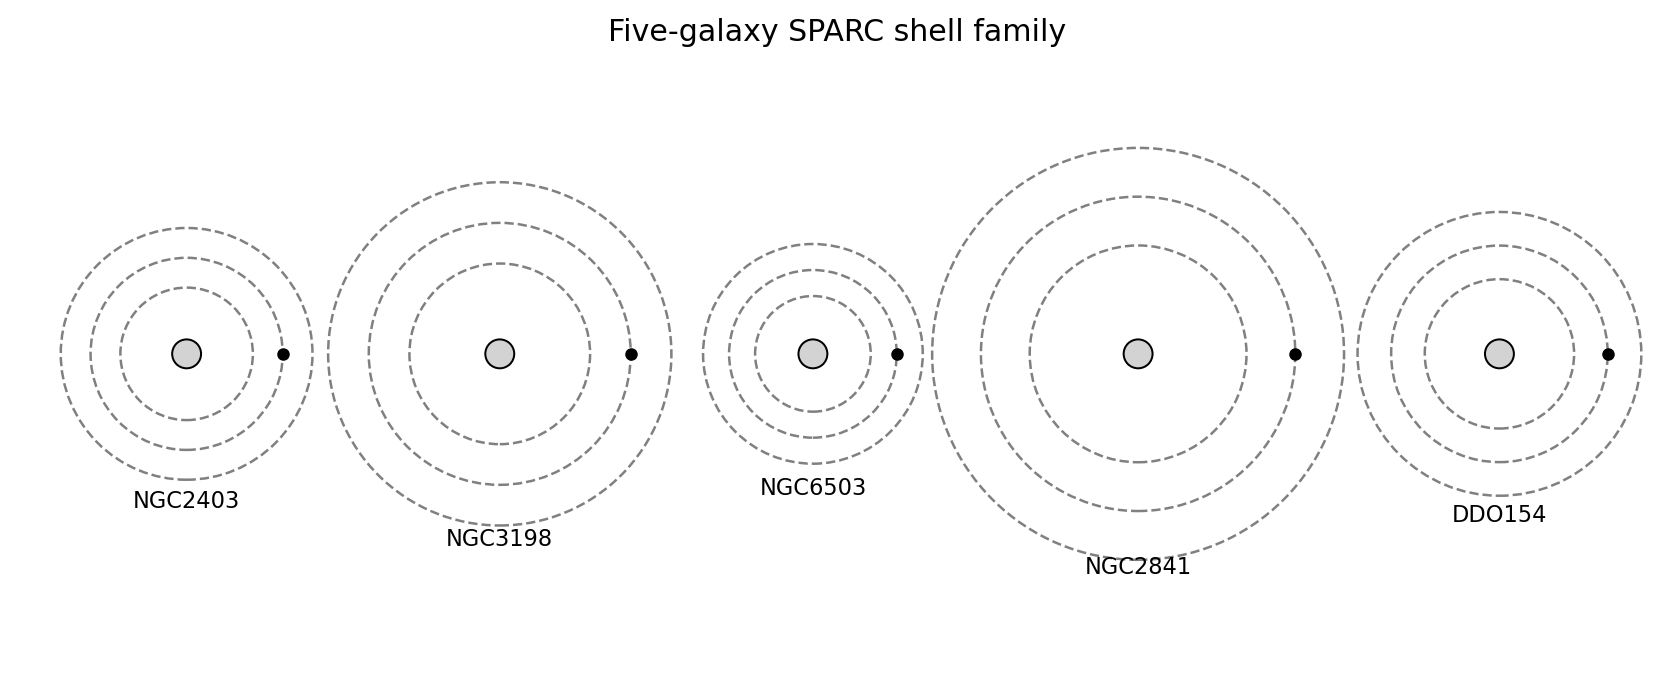
\includegraphics[width=0.88\linewidth]{figures/galactic/sparc5_shell_family.png}
\caption{Five-galaxy SPARC shell family with extracted star slices. The visible shell/ring layout is regenerated from the companion notebook and stored once under the supplement-wide figures directory.}
\end{figure}

\begin{figure}[H]
\centering
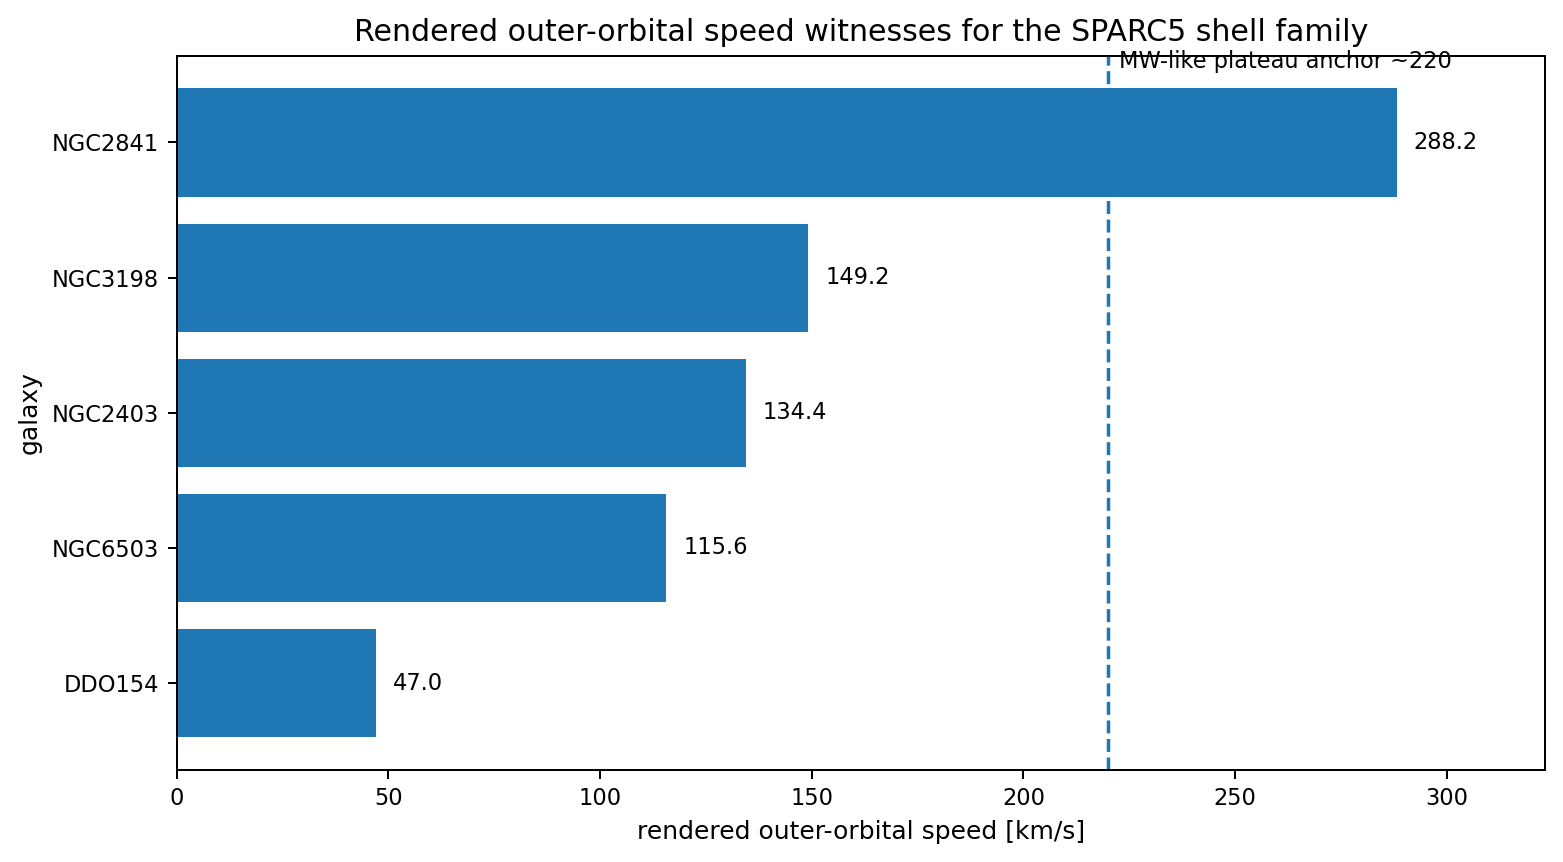
\includegraphics[width=0.88\linewidth]{figures/galactic/sparc5_speed_witnesses.png}
\caption{Calculated and observed outer-orbital speed witnesses for the five cited SPARC galaxies. The comparison is attached only after the cited row has been fixed.}
\end{figure}

\FloatBarrier

\paragraph{Hook / Evidence.} Use the cited long-window drift and support hooks. The SPARC database and the long-baseline rotation-curve review are render-layer anchors for the converted comparison only.

\paragraph{Companion notebook and manifest.} See Section~\ref{app:suppc-notebooks} for the executed calculation manifest and generated figure provenance for this section.

\begin{quote}\small\path{notebooks/galactic/c6_sparc5_shells_worked.ipynb}\end{quote}
